\chapter{Low-Code}
    \begin{displayquote} \centering
        \say{\textit{The future of coding is no coding at all.}} \\
        \hspace*{\fill}---Chris Wanstrath, Co-Founder, Github
    \end{displayquote}
    \vspace{1em}

    Σε αυτό το κεφάλαιο, περιγράφεται η έννοια του low-code (χαμηλός κώδικας). Αναφερόμαστε στον ορισμό του, στην ιστορική εξέλιξη της μηχανικής λογισμικού που επέτρεψε την ύπαρξη πλατφορμών ανάπτυξης λογισμικού σε low-code...

    \section{Τι είναι ο χαμηλός κώδικας}
        \begin{displayquote} \justifying
            \say{\textit{When you can visually create new business applications with minimal hand-coding --when your developers can do more of greater value, faster-- that’s low-code.}} \cite{Ibm_2024}
        \end{displayquote}

        Για να κατανοήσουμε καλύτερα την έννοια του χαμηλού κώδικα, μπορούμε να εξετάσουμε την εξέλιξη των γλωσσών προγραμματισμού. Για παράδειγμα, η Python, μια γλώσσα υψηλού επιπέδου, θα μπορούσε να χαρακτηριστεί ως χαμηλός κώδικας σε σύγκριση με τη C++. Αντίστοιχα η C θα μπορούσε να χαρακτηριστεί και αυτή χαμηλός κώδικας συγκριτικά με την Assembly, όπως και η Assembly είναι χαμηλός κώδικας αν τη συγκρίνουμε με το να αλλάζουμε χειροκίνητα μηδενικά και άσσους στους καταχωρητές. Πρακτικά, η εξέλιξη του προγραμματισμού ταυτίζεται με την εξέλιξη του χαμηλού κώδικα.

        Επομένως, ο χαμηλός κώδικας, αν και ονομάστηκε πρόσφατα ως όρος, η \textit{έννοιά} του δεν είναι καθόλου καινούρια, και είναι η άμεση εξέλιξη του υψηλού επιπέδου γλωσσών προγραμματισμού (4GLs) των τελευταίων δεκαετιών. Το υψηλότερο προγραμματιστικό επίπεδο με τις αφαιρέσεις που διαθέτει, επιτρέπει ευκολότερη και γρηγορότερη ανάπτυξη λογισμικού. Πέρα όμως από τους χρήστες που είναι ήδη προγραμματιστές, προσφέρει επιπλέον τη δυνατότητα σε χρήστες με λίγη ή και καθόλου προγραμματιστική εμπειρία\footnote{Αποκαλούμενοι ως \textbf{citizen developers} (προγραμματιστές πολίτες), πρόκειται για χρήστες με λίγη ή μηδενική προγραμματιστική εμπειρία που χρησιμοποιούν προγραμματιστικά εργαλεία χαμηλού κώδικα για τον σχεδιασμό εφαρμογών (περιγράφονται αναλυτικότερα στο \ref{subsec:citizen-developer}).} να τροποποιήσουν εφαρμογές ή και να φτιάξουν εξ' ολοκλήρου τις δικές τους, με την ίδια λογική όπως η Python επέτρεψε σε περισσότερο κόσμο να προγραμματίσει σε σχέση με την Assembly. Ο προγραμματισμός σε χαμηλό κώδικα πραγματοποιείται σε πλατφόρμες που ονομάζονται \textbf{Πλατφόρμες Ανάπτυξης Λογισμικού σε Low-Code} (Low-Code Development Platforms -- LCDPs), οι οποίες θα αναλυθούν εκτενέστερα στα επόμενα κεφάλαια. Οι πλατφόρμες περιλαμβάνουν γραφικό περιβάλλον με drag-and-drop και WYSIWYG (What-You-See-Is-What-You-Get) editors, επιτρέποντας την πιο γρήγορη και ενστικτώδη κατασκευή εφαρμογών. Αυτός ο οπτικός προγραμματισμός (visual programming) είναι σημαντικός παράγοντας στην προσβασιμότητα που προσφέρει ο χαμηλός κώδικας. \cite{LowCodeMendix} \cite{LowCodeSimon} \cite{LowCodeDemocratization}

            \subsection{Οπτικός προγραμματισμός (visual programming)}
                Παρακάτω παρατίθενται δύο παραδείγματα από την παραδοσιακή ανάπτυξη εφαρμογών και την ανάπτυξη εφαρμογών σε low-code στην πλατφόρμα Mendix.

                \begin{figure}[H] \noindent \centering
                        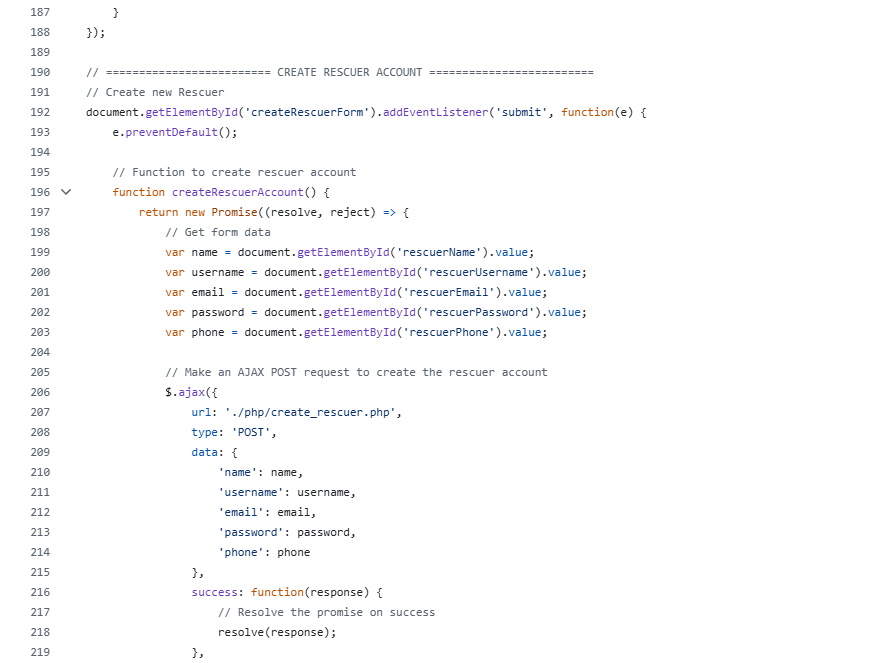
\includegraphics[trim={0 15cm 0 3cm}, clip, width=0.8\textwidth]{ClassicProgramming}
                        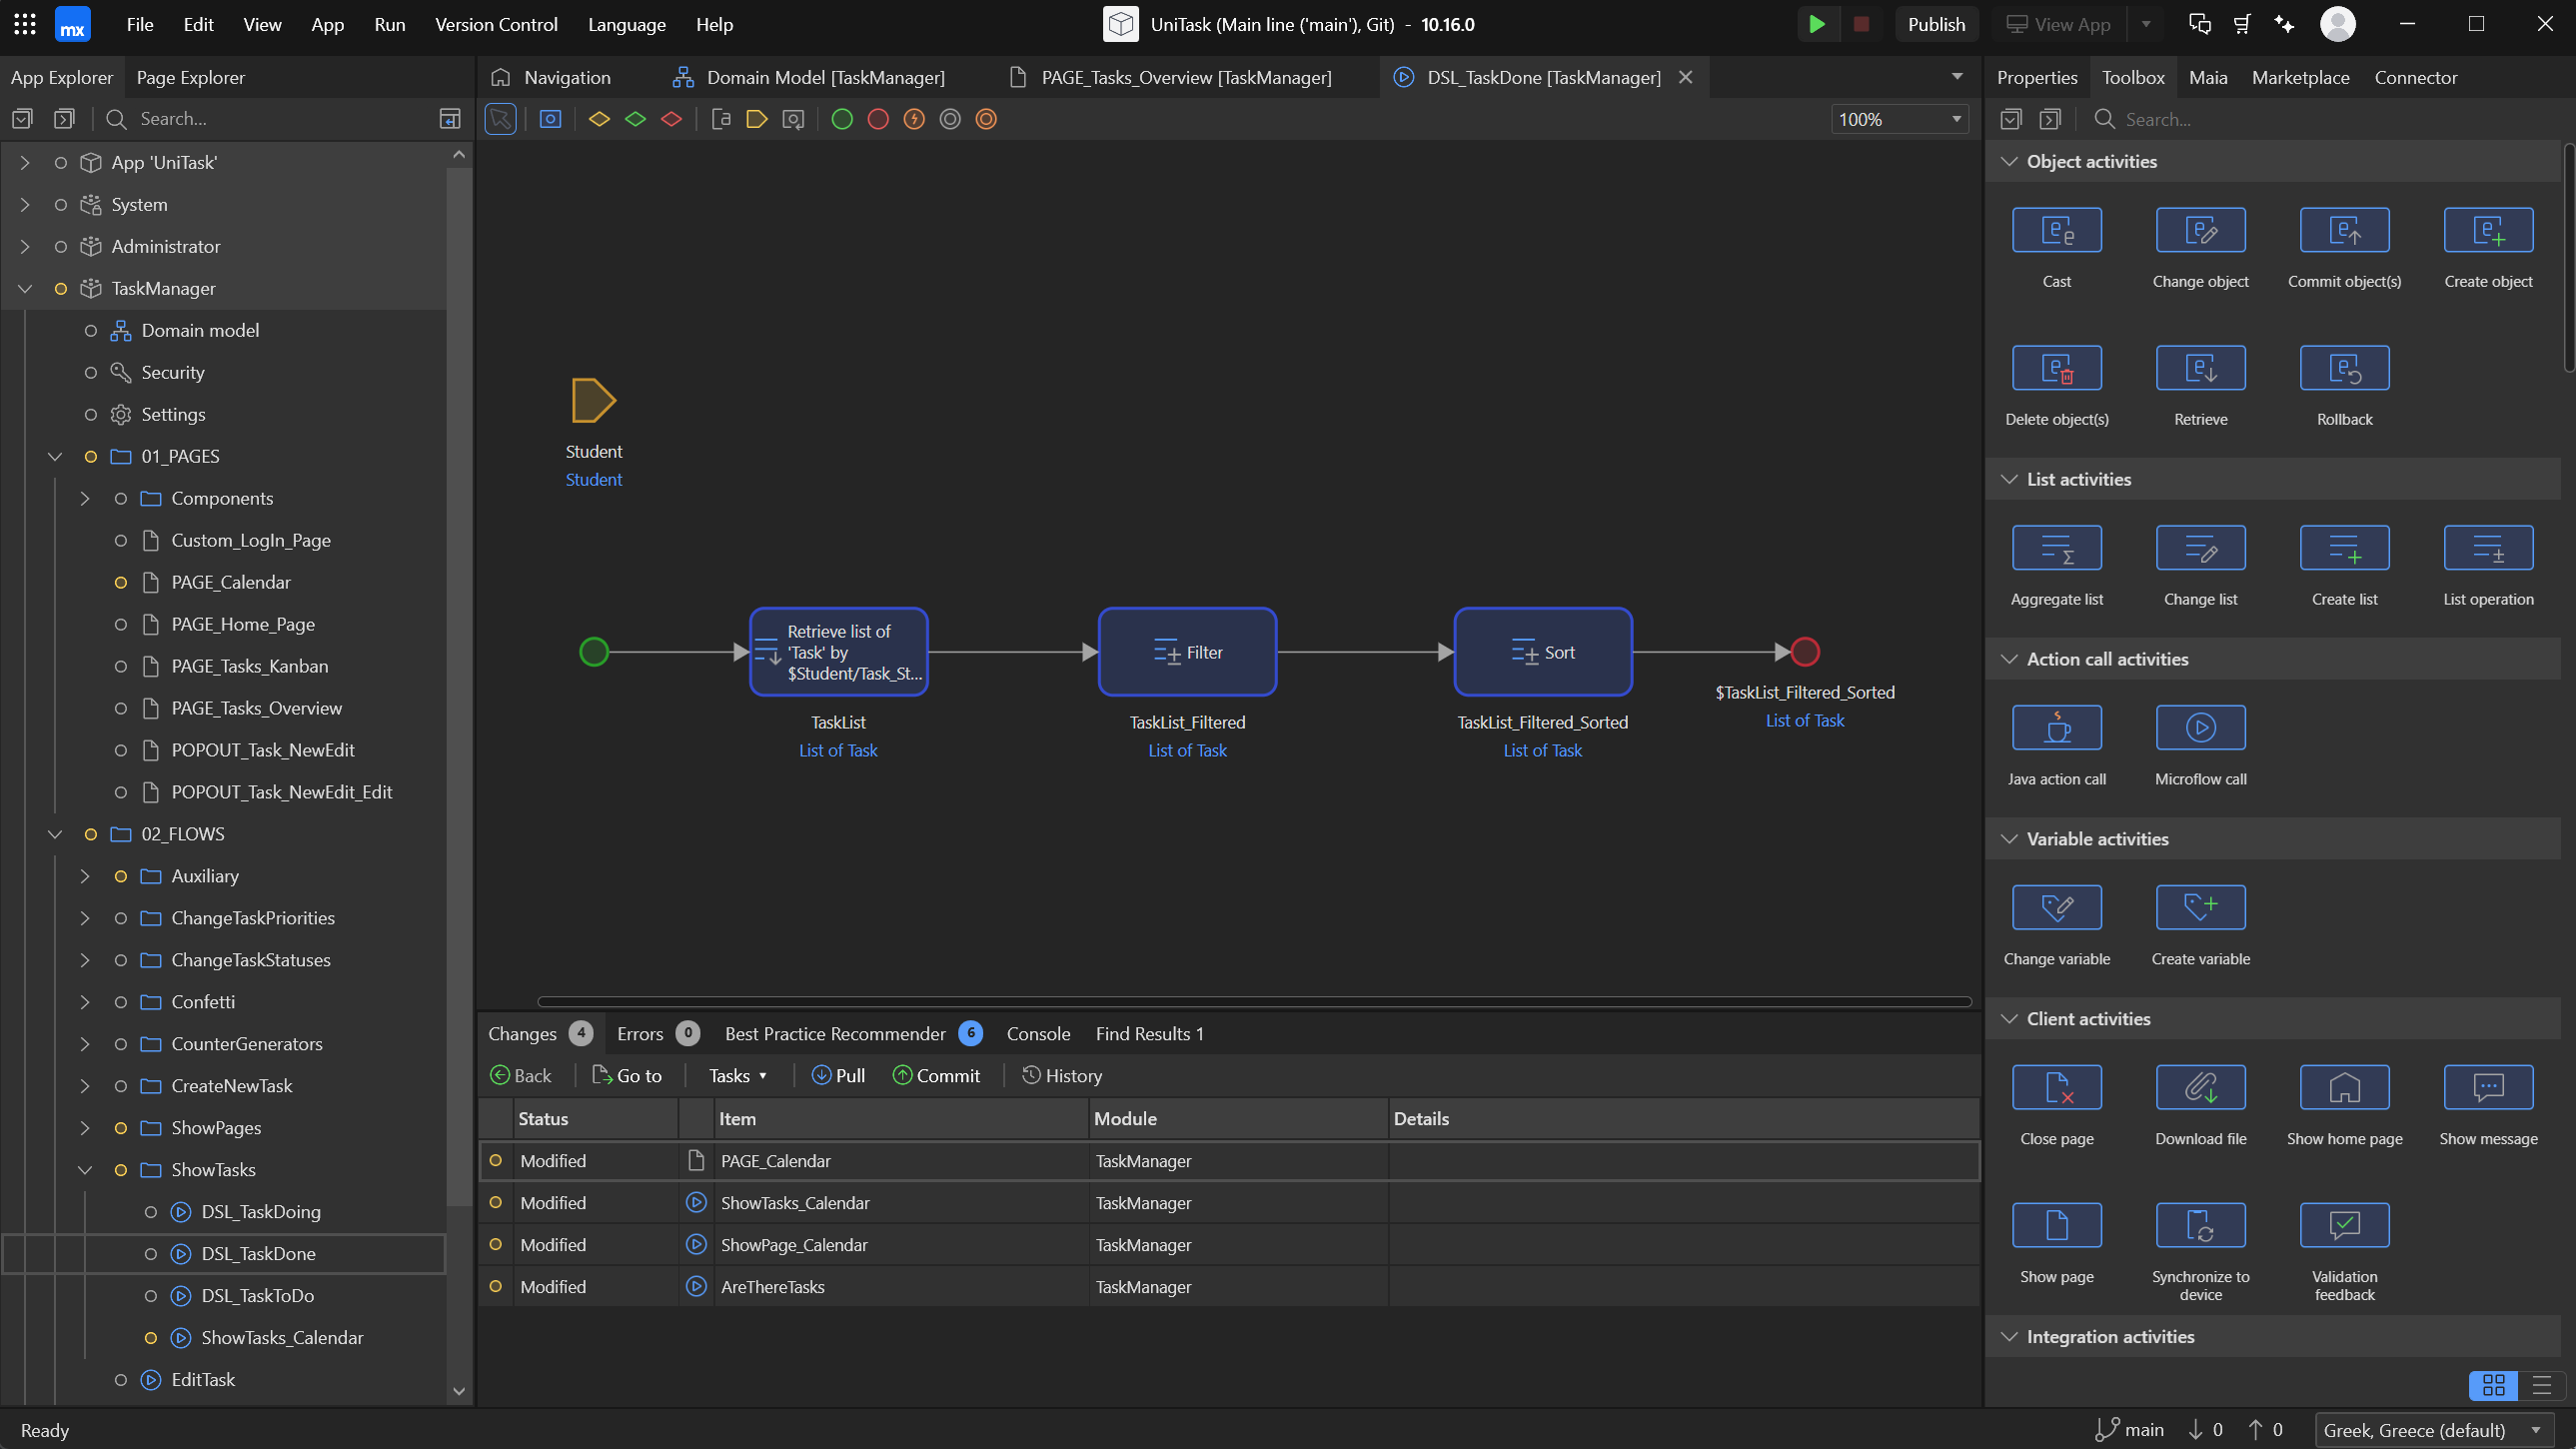
\includegraphics[trim={0 0 0 0}, clip, width=0.8\textwidth]{MendixLowCodeDevelopment}
                        \caption{Παραδοσιακός κώδικας και το γραφικό περιβάλλον του Mendix.}
                        \label{fig:codevsmendix}
                \end{figure}

                Στο γραφικό περιβάλλον ο προγραμματισμός γίνεται σε ένα διάγραμμα ροής με drag-and-drop επαναχρησιμοποιούμενα στοιχεία (εν προκειμένω στο σχήμα \ref{fig:codevsmendix}, ένα παράδειγμα επαναχρησιμοποιούμενων στοιχείων είναι τα μπλε τετράγωνα στο διάγραμμα ροής και δεξιά της οθόνης), σε αντίθεση με τον παραδοσιακό κώδικα όπου γράφουμε γραμμή-γραμμή, κάτι που καθιστά την ανάπτυξη εφαρμογών εξαιρετικά γρήγορη και προσβάσιμη από περισσοτέρους.

                Η οπτικοποίηση του προγραμματισμού πρόκειται για μια εκ θεμελίων επαναστατική αλλαγή. Εξάλλου, τα πετρογραφικά και οι ζωγραφιές στους τοίχους παλαιών σπηλαίων είναι ένα δείγμα από το πόσο ουσιώδης ήταν πάντα η οπτική επικοινωνία για τον άνθρωπο. \cite{CASEKuhn}  Ο οπτικός προγραμματισμός τους επιτρέπει να προσθέτουν λειτουργικότητες χειριζόμενοι γραφικά στοιχεία αντί να τα προσδιορίζουν μέσω κειμένου. Πέρα από αυτό, οι απλοί χρήστες συνήθως θεωρούν το ποντίκι πολύ πιο προσβάσιμο από το πληκτρολόγιο.

            \subsection{Καθόλου κώδικας (no-code)}
                Ένας εύληπτος τρόπος για να καταλάβουμε τη διαφορά ανάμεσα στον χαμηλό κώδικα με τον καθόλου κώδικα είναι το γεγονός πως στα no-code εργαλεία οι χρήστες δε χρησιμοποιούν καθόλου το πληκτρολόγιό τους. Όλη η αλληλεπίδραση με το λογισμικό πραγματοποιείται με το ποντίκι μέσω του γραφικού περιβάλλοντος. Ο περιοριστικός χαρακτήρας αυτών των εργαλείων έχει ως πλεονέκτημα το ότι οι χρήστες είναι δύσκολο να δημιουργήσουν σφάλματα, αλλά το μειονέκτημα είναι το ότι δεν υπάρχει η δυνατότητα εξατομικευμένης παραμετροποίησης από τον χρήστη.

                Να σημειωθεί πως ο χαμηλός κώδικας περιλαμβάνει τα οφέλη και του κλασικού προγραμματισμού και του καθόλου κώδικα, αφού ο χρήστης διαθέτει την επιλογή να χρησιμοποιήσει τα έτοιμα εργαλεία της πλατφόρμας ή και να δημιουργήσει το δικό του κώδικα και να παραμετροποιήσει ό,τι ακριβώς θέλει αυτός.

            \begin{figure}[H] \noindent \centering
                    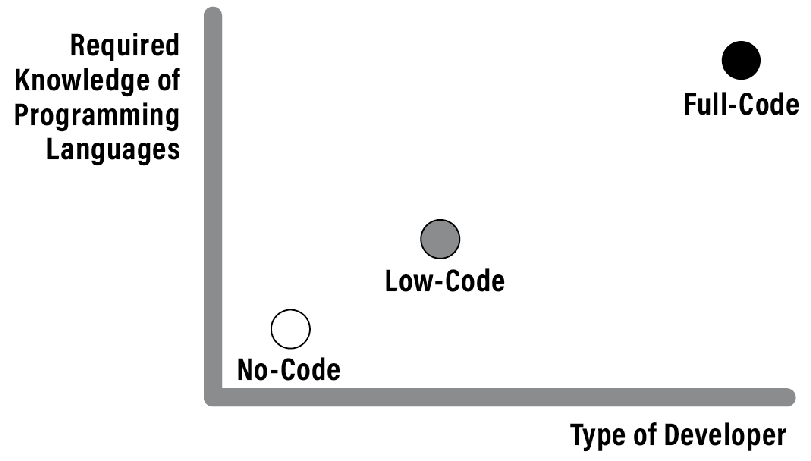
\includegraphics[width=0.7\textwidth]{DeveloperVsCode}
                    \caption{\centering Σύγκριση ανάμεσα στην προγραμματιστική εμπειρία των χρηστών \\ και την προγραμματιστική προσέγγιση που χρησιμοποιούν \cite{LowCodeSimon}}
            \end{figure}

            \subsection{Η έννοια του προγραμματιστή πολίτη (citizen developer)} \label{subsec:citizen-developer}
                Ο προγραμματιστής πολίτης είναι ένας χρήστης που αναπτύσσει εφαρμογές σε συνεργασία με τους προγραμματιστές, χωρίς να είναι απαραίτητο να διαθέτει προγραμματιστικές γνώσεις. Η έλλειψη προηγούμενων γνώσεων και εμπειρίας στον προγραμματισμό δεν τον εμποδίζει από το να συνεισφέρει στην ανάπτυξη με ισότιμο τρόπο όπως οι παραδοσιακοί προγραμματιστές.

                Μια περίληψη των βασικών διαφορών που παρατηρούνται ανάμεσα στους προγραμματιστές πολίτες και τους μηχανικούς λογισμικού συνοψίζεται στον παρακάτω πίνακα \cite{LowCodeSimon}:

                \begin{table}[H] \noindent\centering
                    \resizebox{\textwidth}{!}{
                        \begin{tabular}{c|c|c}
                           \textbf{Χαρακτηριστικό} & \textbf{Παραδοσιακός μηχανικός λογισμικού} & \textbf{Προγραμματιστής πολίτης} \\
                            \midrule
                            Γνωστικό & Μηχανική λογισμικού ή & Ποικίλει \\
                            υπόβαθρο & Επιστήμη των Υπολογιστών & \\
                            \midrule
                            Θέση στην & Τεχνολογία πληροφοριών (IT), & Μάρκετινγκ, πωλήσεις, \\
                            επιχείρηση & DevOps & HR, λογιστικά \\
                            \midrule
                            Γνώσεις που αφορούν & Λίγες & Πολλές \\
                            την επιχείρηση & & \\
                        \end{tabular}}
                \end{table}

                Ο ρόλος των προγραμματιστών πολιτών προβλέπεται να εκτιναχθεί στα επόμενα χρόνια, όχι τόσο ως μια καινούρια θέση εργασίας αλλά παραπάνω ως ένα επιπλέον χαρακτηριστικό στις υπάρχουσες θέσεις. Η Gartner\footnote{Η Gartner είναι μια διεθνώς αναγνωρισμένη εταιρία ερευνών και συμβουλευτικών υπηρεσιών με κύριους πελάτες της οργανισμούς στους τομείς της τεχνολογίας, της επιχειρηματικής στρατηγικής και της καινοτομίας. Πρόκειται για έναν από τους πιο έγκυρους φορείς για αναλύσεις σε τάσεις στο τομέα της πληροφορικής και της τεχνολογίας.} αναφέρει πως \say{ως το 2023, ο αριθμός των ενεργών προγραμματιστών πολιτών σε μεγάλες επιχειρήσεις θα είναι τουλάχιστον τετραπλάσιος από τοιν αριθμό των παραδοσιακών προγραμματιστών} \cite{GartnerReport} ενώ η Microsoft αναφέρει πως \say{οι προγραμματιστές πολίτες θα αναπτύξουν 450 εκατομμύρια εφαρμογές το 2025 χρησιμοποιώντας χαμηλό ή καθόλου κώδικα} \cite{cnbcNextFrontier}.

                \subsubsection{Διαφορά με τους παραδοσιακούς προγραμματιστές}
                    Οι παραδοσιακοί προγραμματιστές, παραδόξως, δεν αντιμετωπίζουν τους προγραμματιστές πολίτες με καχυποψία αλλά με ενθουσιασμό. Ο λόγος είναι απλός και συνοψίζεται στο σχήμα \ref{fig:DevVSCitDev}. Όσο εντυπωσιακές και αν είναι οι ικανότητες των προγραμματιστών πολιτών, παραμένει ανέφικτο για αυτούς να σχεδιάσουν πολύπλοκα συστήματα για επιχειρήσεις. Οι παραδοσιακοί προγραμματιστές και μηχανικοί λογισμικού είναι αυτοί που μπορούν, και με το βάρος των αδιάφορων λεπτομερειών και του troubleshooting να έχει φύγει από πάνω τους και να έχει μετακινηθεί στους προγραμματιστές πολίτες, μπορούν και εστιάζουν περισσότερο στον σχεδιασμό και την αρχιτεκτονική των εφαρμογών.

                    \begin{figure}[h!] \noindent \centering
                            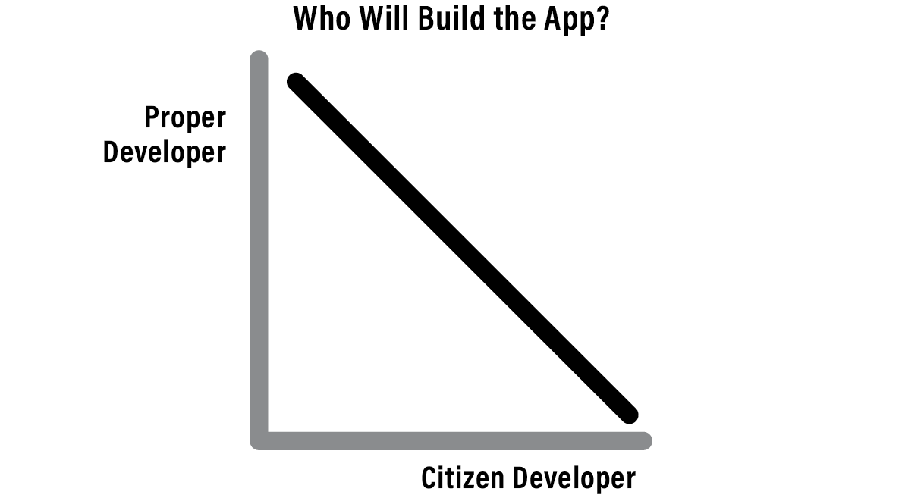
\includegraphics[width=0.7\textwidth]{DevVSCitDev}
                            \caption{Ποιος θα φτιάξει την εφαρμογή; \cite{LowCodeSimon}}
                            \label{fig:DevVSCitDev}
                    \end{figure}

                \subsubsection{Χαρακτηριστικά των προγραμματιστών πολιτών}
                    Σε έρευνα \cite{QuickBaseCitizenDevReport} που πραγματοποίησε το QuickBase ανάμεσα σε 148 αυτοαποκαλούμενους προγραμματιστές πολίτες, το 97\% κατείχε βασικές ικανότητες επεξεργασίας κειμένου και υπολογιστικών φύλλων, το 36\% κατείχε βασικές γνώσεις σε front-end web development (HTML, CSS και Javascript), ενώ το 8\% είχε επαφή με Java, .NET, Python, Ruby, PHP και άλλες γλώσσες προγραμματισμού.

                    \begin{figure}[H] \noindent \centering
                            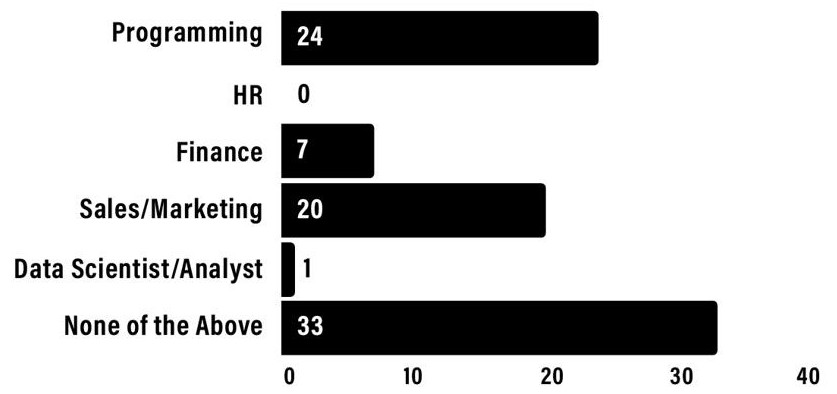
\includegraphics[width=0.6\textwidth]{CitDevBg}
                            \caption{Επαγγελματικό υπόβαθρο προγραμματιστών πολιτών. \cite{LowCodeSimon}}
                    \end{figure}

                    \vspace{-2.5em}
                    \begin{displayquote}
                        \small Έχει ενδιαφέρον ότι το 72\% των συμμετεχόντων δεν είναι προγραμματιστές αλλά έχουν διαφορετικό επαγγελματικό αντικείμενο. Από την άλλη το 28\% των συμμετεχόντων οι οποίοι είναι προγραμματιστές φανερώνει μια τάση ότι και οι ίδιοι οι προγραμματιστές χρησιμοποιούν εργαλεία χαμηλού κώδικα.
                    \end{displayquote}

                    \begin{figure}[H] \noindent \centering
                            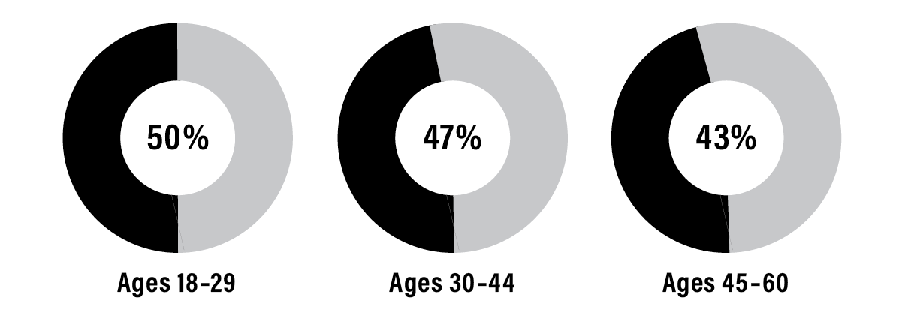
\includegraphics[width=0.7\textwidth]{CitDevAge}
                            \caption{Ηλικιακή κατανομή προγραμματιστών πολιτών. \cite{CitDevTrackVia}}
                    \end{figure}

                    \vspace{-2.5em}
                    \begin{displayquote}
                        \small Υπάρχει τάση οι νεότεροι ηλικιακά να έχουν μεγαλύτερες πιθανότητες να είναι προγραμματιστές πολίτες.
                    \end{displayquote}


    \section{Πώς φτάσαμε στον χαμηλό κώδικα}
        Θα επεκταθούμε στα επόμενα κεφάλαια στα οφέλη του low-code και στα χαρακτηριστικά των πλατφορμών ανάπτυξης λογισμικού σε low-code. Πριν προχωρήσουμε, αξίζει να εξετάσουμε πρώτα τις τεχνολογικές εξελίξεις που μας οδήγησαν σήμερα σε αυτές τις πλατφόρμες.

        Η μηχανική λογισμικού\footnote{Θα ορίζαμε τη μηχανική λογισμικού ως μια πειθαρχημένη και αυστηρή εφαρμογή μεθόδων, διαδικασιών και εργαλείων στη διαχείριση και ανάπτυξη υπολογιστικών συστημάτων. Πρόκειται για ένα εννοιλογικό πλαίσιο που περιγράφει τη διαχείριση συστημάτων.} έχει περάσει πολλά στάδια στην ιστορία της μέχρι να αρχίσουμε να αναφερόμαστε και σε χρήση χαμηλού κώδικα. Μέχρι τη δεκαετία του 1970, η ανάπτυξη πληροφοριακών συστημάτων έμοιαζε παραπάνω ως μια τέχνη παρά ως επιστήμη, καθώς δεν ακολουθούσε κάποια δόμηση. Αντιθέτως, ο προγραμματιστής λάμβανε μια σειρά από απαιτήσεις και ανάγκες από την πλευρά του χρήστη, και μετά από ένα διάστημα παρέδιδε ένα σύστημα που συνήθως δεν κάλυπτε εξ ολοκλήρου όλες τις απαιτήσεις του χρήστη αλλά ήταν σίγουρα καλύτερο από το τίποτα. Η συγκεκριμένη μέθοδος, αποκαλούμενη \textbf{κλασική μέθοδος}, χαρακτηρίζεται από ανεπίσημες οδηγίες, έλλειψη τυποποίησης και αναφορών (documentation).

        Η ανάγκη για αύξηση της παραγωγικότητας στον κύκλο ζωής έκδοσης λογισμικού (software release life cycle)\footnote{Πρόκειται μια έννοια που αναφέρεται στις φάσεις ανάπτυξης και ύπαρξης ενός λογισμικού. Ξεκινάει από τη σύλληψη της ιδέας, τη μελέτη για τις απαιτήσεις του, την υλοποίηση του, τη διάθεση του προϊόντος στο πελάτη, τη υποστήριξή του με ενημερώσεις και τέλος την απόσυρσή του.} οδήγησε στη δημιουργία \textbf{επίσημων μεθόδων} στα τέλη της δεκαετίας του 1970. Σκοπός τους ήταν η τυποποίηση του σχεδιασμού με στόχο τη βελτίωση της ποιότητάς του. Παράδειγμα αυτών των τεχνικών είναι η χρήση δομημένης ανάλυσης (structured analysis). Έτσι, οι μηχανικοί μπορούσαν να φτιάξουν διαγράμματα ροών δεδομένων (data flow diagrams)\footnote{Είναι μια οπτική αναπαράσταση της ροής των δεδομένων σε ένα σύστημα. Αναγράφονται οι διεργασίες (κύκλοι), οι είσοδοι και έξοδοι (τετράγωνα) και η αποθήκευση των δεδομένων (παράλληλες γραμμές).}, μοντέλα οντοτήτων-συσχετίσεων (ER -- entity-relationship models)\footnote{Περιγράφει ένα σύνολο αντικειμένων (οντότητες) και τις \textit{σχέσεις} μεταξύ αυτών των αντικειμένων.}, δημιουργώντας μια συστημική περιγραφή του λογικού και φυσικού μέρους του πληροφοριακού συστήματος που ανέπτυσσαν.

        Με την περαιτέρω ανάπτυξη των προσωπικών υπολογιστών στα μέσα της δεκαετίας του 1980, η χρήση επίσημων μεθόδων ήταν μονόδρομος, και μάλιστα δημιούργησε μια νέα τάση, την ανάγκη για αυτοματοποίηση της ανάπτυξης κώδικα και την ελαχιστοποίηση της χειροκίνητης γραφής του.

        Απόρροια αυτής της τάσης ήταν α) τη δεκαετία του 1980 οι \textbf{γλώσσες προγραμματισμού τέταρτης γενιάς} (4GLs)\footnote{Σε αντίθεση με τις γλώσσες προγραμματισμού τρίτης γενιάς (C, Java κτλ) που σε αντίθεση με της δεύτερης (Assembly) επέτρεπαν τη δημιουργία προγραμμάτων ανεξάρτητα από το μηχάνημα που θα τις έτρεχε, οι γλώσσες προγραμματισμού τέταρτης γενιάς σχεδιάστηκαν με γνώμονα την απλοποίηση του προγραμματισμού. Χαρακτηρίζονται από υψηλού επιπέδου αφαιρέσεις, πλησιάζοντας στην ανθρώπινη γλώσσα, κάνοντάς τες πιο εύκολα κατανοητές. Παραδείγματα είναι η Python, SQL, Ruby.}, τα \textbf{Computer-Aided Software Engineering} (CASE) περιβάλλοντα, β) η \textbf{Ταχεία Ανάπτυξη Εφαρμογών} (Rapid Application Development -- RAD)\footnote{Πρόκειται για μια μεθοδολογία που δίνει βάση στη δημιουργία πρωτοτύπων. Έτσι οι προγραμματιστές δε χρειάζεται να ξεκινάνε από το μηδέν την ανάπτυξη κάθε νέου λογισμικού, ούτε να ξοδεύουν πολύτιμο χρόνο για να περιγράψουν λεπτομερώς όλες τις προδιαγραφές του. Χρησιμοποιώντας έτοιμα (μάλιστα και modular) πρωτότυπα, ο χρόνος ανάπτυξης μειώνεται. Παραδείγματα RAD εργαλείων είναι οι GUI builders· πρόκειται για WYSIWYG (What-You-See-Is-What-You-Get) επεξεργαστές για τη γρήγορη ανάπτυξη λογισμικών με διεπαφή χρήστη (user interface).} τη δεκαετία του 1990, γ) ο \textbf{Προγραμματισμός τελικού χρήστη} (End-User Development -- EUD)\footnote{Περιγράφει εργαλεία που επιτρέπουν τον προγραμματισμό από τους απλούς τελικούς χρήστες. Παραδείγματα είναι λογιστικά φύλλα όπως το Microsoft Excel ή εκπαιδευτικά εργαλεία όπως το Scratch.} τη δεκαετία του 2000, και οι \textbf{αρχιτεκτονικές που βασίζονται σε μοντέλα} (model-driven architecture -- MDA) τις τελευταίες δύο δεκαετίες. \cite{Case1985, CASEChikofsky, MDELow}

        Στις επόμενες υποενότητες θα αναφερθούμε πιο εκτεταμένα στα CASE και MDA περιβάλλοντα, τα οποία υπήρξαν και τα κύρια πρωταίτια των Low-Code περιβαλλόντων.

        \subsection{Computer-Aided Software Enginnering (CASE)}
            Τα \textbf{Computer-Aided Software Engineering} (CASE -- Μηχανική Λογισμικού Υποβοηθούμενη από Υπολογιστή) περιβάλλοντα επέτρεπαν τους μηχανικούς να καταγράφουν και να μοντελοποιούν με συστηματικό τρόπο ένα πληροφοριακό σύστημα από τις αρχικές περιγραφές του χρήστη ως τη σχεδίαση και την υλοποίηση και να εκτελούν δοκιμές για τη συνέπειά του.

            Μέχρι πρότινος, τα εργαλεία που αφορούν την ανάπτυξη λογισμικού εστιάζουν κυρίως στην επεξεργασία πηγαίου κώδικα και την αποσφαλμάτωση του. Σε αντίθεση λοιπόν με τα υπάρχοντα εργαλεία, τα CASE περιβάλλοντα επικεντρώνονται στη \textit{μεθοδολογία} της ανάπτυξης λογισμικού: στην ανάλυση απαιτήσεων, στο λογικό σχεδιασμό, στον έλεγχο εγκυρότητας, την επαναχρησιμοποίηση και εξάλειψη πλεονασμών.

            Είναι το δεξί χέρι ενός μηχανικού λογισμικού, βοηθώντας σε πολλές εργασίες που τον δυσκολεύουν, αυξάνοντας την παραγωγικότητα και την ποιότητα της δουλειάς του. Τα εργαλεία που περιλαμβάνουν ποικίλλουν: κάποια επιτρέπουν τη δημιουργία διαγραμμάτων ενώ άλλα μπορούν να αυτοματοποιούν όλα τα στάδια του κύκλου ζωής έκδοσης λογισμικού. Ένα ολοκληρωμένο CASE περιβάλλον περιλαμβάνει:
            \vspace{-0.5em}
            \begin{itemize}[label={\tiny \blacksquare}]
                \setlength\itemsep{-0.25em}
                \item ένα διαδραστικό και φιλικό για το χρήστη γραφικό περιβάλλον διαχείρισης
                \item ένα σύνολο από εργαλεία ανάπτυξης (επεξεργαστές κειμένου, λεξικά, αναλυτές σχεδιασμού κ.α.)
                \item ένα σύνολο από εργαλεία για τον έλεγχο της διαδικασίας (για τον χρονοπρογραμματισμό, τη διασφάλιση ποιότητας κ.α.)
                \item ένα περιβάλλον βοήθειας με το documentation των εργαλείων
                \item ένα σύστημα διαχείρισης βάσεων δεδομένων
            \end{itemize}
            \vspace{-0.5em}

            Τα συστήματα που δημιουργούνται από το CASE είναι εφαρμογές της πειθαρχημένης εφαρμογής μεθόδων της μηχανικής λογισμικού.
            Τα CASE περιβάλλοντα έθεσαν τα θεμέλια για τη δημιουργία νέων προτύπων, όπως ο οπτικός προγραμματισμός (visual programming) και ο προγραμματισμός που βασίζεται σε μοντέλα. \cite{CASEChikofsky, Case1985, CASEKuhn, AdoptionCASE}

        \subsection{Model-driven Architecture (MDA)}
            Τα μοντέλα προσφέρουν τη δυνατότητα αφαίρεσης σε ένα σύστημα, κάτι που επιτρέπει τους μηχανικούς να επικεντρώνονται μόνο στο πρόβλημα που προσπαθούν να λύσουν, αγνοώντας τις υπόλοιπες λεπτομέρειες. Η χρήση μοντέλων είναι απαραίτητα για την κατανόηση και επεξεργασία πολύπλοκων συστημάτων. Ένα παράδειγμα μοντελοποίησης, για παράδειγμα, θα μπορούσε να είναι τα διαφορετικά επίπεδα εμφάνισης ενός συστήματος (δομικό επίπεδο, επίπεδο συμπεριφοράς κα).

            Η ιδέα των μοντέλων αποτέλεσε τη βάση για μια νέα προσέγγιση ανάπτυξης λογισμικού, τη \textit{μηχανική που βασίζονται σε μοντέλα} (model-driven engineering -- MDE). Μπορούμε να περιγράψουμε με σαφήνεια και με κανόνες τα μοντέλα (για παράδειγμα το πως θα μετατραπεί ένα μοντέλο σε ένα άλλο, την παρακολούθηση μεταξύ στοιχείων ενός μοντέλου κτλ), συντελώντας πλέον στην \textbf{αρχιτεκτονική που βασίζεται σε μοντέλα} (model-driven architecture -- MDA).

            Η MDA υποστηρίζεται από την Object Management Group (OMG) \cite{OMG_MDA}, βασίζεται σε ένα σύνολο προτύπων για τον ορισμών μοντέλων, συμβολισμών και κανόνων μετασχηματισμού και προσφέρει μια βάση για τη λειτουργία μοντέλων όπως το UML. Τα μοντέλα χρησιμοποιούνται για τον προσδιορισμό, την προσομοίωση, την επαλήθευση, τον εκσυγχρονισμό, τη συντήρηση, την κατανόηση και τη δημιουργία κώδικα. Στόχος παραμένει η αυτοματοποίηση διαφόρων βημάτων στην ανάπτυξη λογισμικού, αυξάνοντας παράλληλα την ποιότητά του. Επιπλέον, χρησιμοποιώντας μοντέλα είναι εφικτός ο διαχωρισμός της λειτουργικότητας των εφαρμογών από την υλοποίησή της σε μια συγκεκριμένη πλατφόρμα. Ως αποτέλεσμα, οι προγραμματιστές μπορούν να εστιάζουν περισσότερο στον σχεδιασμό και λιγότερο στο να λύνουν θέματα που αφορούν την πλατφόρμα υλοποίησης.

            Εν τέλει, η αρχιτεκτονική που βασίζεται σε μοντέλα άλλαξε τον τρόπο σκέψης των προγραμματιστών, καθώς πλέον επικεντρώνονταν παραπάνω στον σωστό διαχωρισμό των χαρακτηριστικών, στην αφαιρετικότητα και στην αυτοματοποίηση.
            \cite{Bucaioni2022, MDELow, MDSDSpringer}

        \subsection{Προγενέστερα λογισμικά οπτικού προγραμματισμού}
            Τα CASE περιβάλλοντα και η μηχανική που βασίζεται σε μοντέλα έφεραν ριζικές αλλαγές στη φιλοσοφία της μηχανικής λογισμικού. Στο κομμάτι του οπτικού προγραμματισμού όμως, δεν ήταν τα LCDP τα πρώτα που περιλάμβαναν ένα γραφικό περιβάλλον εργασίας. Το Microsoft Access ήταν ένα από τα πρώτα λογισμικά που πρόσφεραν γραφικό περιβάλλον εργασίας. Οι χρήστες σέρνοντας και αφήνοντας στοιχεία μπορούσαν να κατασκευάζουν βάσεις δεδομένων, φόρμες κ.α. χωρίς την ανάγκη της SQL.

            \begin{figure}[h!] \noindent \centering
                    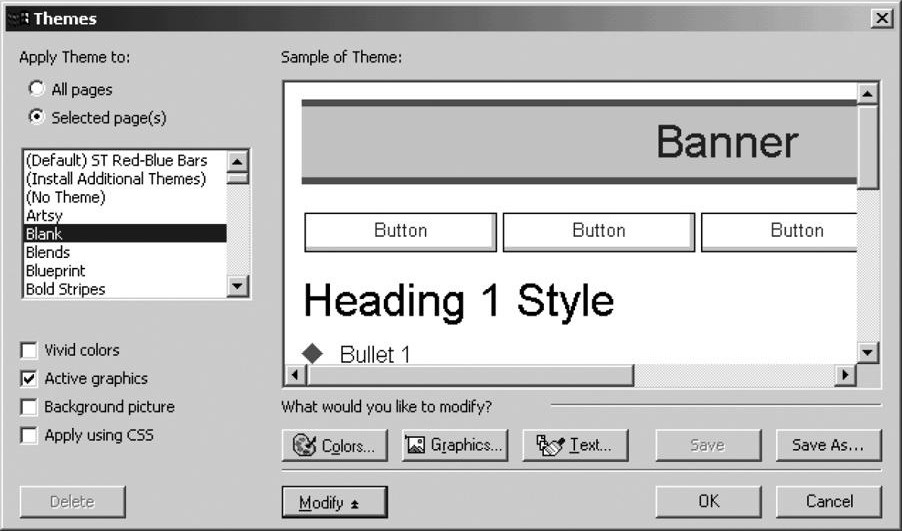
\includegraphics[width=0.6\textwidth]{MicrosoftFrontPage}
                    \caption{\centering Το γραφικό περιβάλλον του Microsoft FrontPage}
            \end{figure}

            Άλλα λογισμικά παρόμοιας λογικής ήταν το Microsoft FrontPage, ένας από τους πρώτους WYSIWYG επεξεργαστές και εργαλεία διαχείρισης ιστοσελίδων, το οποίο όμως γρήγορα έγινε παρωχημένο. Τα λογισμικά αυτά αντικαταστάθηκαν από ένα νέο τύπο λογισμικών, φιλικών προς το χρήστη, με προσβάσιμα και εύληπτα εργαλεία από όλους, τα LCDP. \cite{LowCodeSimon}

    \section{Πλατφόρμες Ανάπτυξης Εφαρμογών σε Low-Code (LCDP)}
        Όσο και αν η έννοια των μοντέλων άλλαξε τη μηχανική λογισμικού και έθεσε νέες προδιαγραφές στον σχεδιασμό του, η εξάρτησή της από δύσχρηστα πρότυπα όπως το UML περιόριζε την ευρεία υιοθέτησή της στη βιομηχανία. Τα τελευταία χρόνια έχουν εμφανιστεί πλατφόρμες χτισμένες πάνω στις αρχές της αφαίρεσης των μοντέλων, που απλοποιούν ακόμη παραπάνω τη διαδικασία της ανάπτυξης. Οι συγκεκριμένες πλατφόρμες ονομάζονται \textbf{Πλατφόρμες Ανάπτυξης Εφαρμογών σε Low-Code} (Low-Code Development Platforms -- LCDPs)\footnote{Εναλλακτικές ονομασίες είναι Low-Code Platforms (LCP), Low-Code Development Platforms (LCDP), ενώ η διαδικασία ανάπτυξης αναφέρεται ως Low-Code Software Development (LCSD). Η έννοια του Low-Code συχνά αναφέρεται και ως Χαμηλός Κώδικας.}.\cite{Bock2021}

        \begin{figure}[H] \noindent \centering
                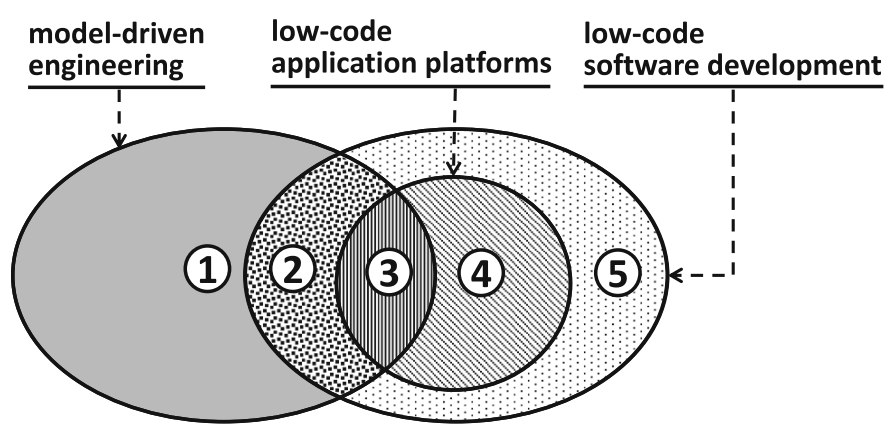
\includegraphics[width=0.6\textwidth]{MDE_LCSD}
                \caption{\centering Σύγκριση μεταξύ της μηχανικής που βασίζεται σε μοντέλα \\ και των Low-Code πλατφορμών. \cite{MDELow}}
        \end{figure}

        \vspace{-2em}
        \begin{displayquote}
            \small Στην περιοχή 1 χρησιμοποιούνται μοντέλα χωρίς να γίνονται προσπάθειες για μείωση του κώδικα, σε αντίθεση με τις περιοχές 2 και 3 που στοχεύουν στην μείωση του κώδικα. Από την άλλη, οι πλατφόρμες ανάπτυξης κώδικα σε low-code δεν βασίζονται πάντα σε μοντέλα (περιοχές 4 και 5), αλλά για παράδειγμα χρησιμοποιούν δεδομένα σε σχεσιακές βάσεις ή σε XML αρχεία. Οι διαφορές μεταξύ low-code application platforms και low-code software development έγκειται στο ότι οι πλατφόρμες προσφέρουν επιπλέον την δυνατότητα διάθεσης του λογισμικού στο ευρύ κοινό, όπως επίσης και την διαχείρισή του καθ' όλο το κύκλο ζωής του.
        \end{displayquote}

        Μια \textbf{Πλατφόρμα Ανάπτυξης Εφαρμογών σε Low-Code} (LCAP) είναι μια πλατφόρμα ανάπτυξης λογισμικού που υποστηρίζει την ταχεία ανάπτυξη και διαχείριση εφαρμογών. Συνήθως είναι Platform-as-a-service (PaaS) cloud μοντέλα, και χρησιμοποιείται ελάχιστος ή και μηδενικός δομημένος προγραμματισμός (structured \linebreak programming).

        Για τον προγραμματισμό παρέχεται γραφικό περιβάλλον με οπτικές αφαιρέσεις (visual abstractions). Έτσι οι προγραμματιστές ή οι citizen developers εστιάζουν παραπάνω στη \textit{σχεδίαση} της εφαρμογής, χωρίς να ξοδεύουν χρόνο άσκοπα σε λεπτομέρειες.

        Με λίγα λόγια, στόχος είναι η αποδοτική ανάπτυξη λογισμικού με τη λιγότερη δυνατή προσπάθεια και με μειωμένο κόστος, και η εύκολη προσαρμογή του λογισμικού στις ταχέως μεταβαλλόμενες συνθήκες των σημερινών λειτουργικών συστημάτων. Η χρήση των LCAP έχει τύχει θετικής αποδοχής από τη βιομηχανία και η υιοθέτησή τους αυξάνεται συνεχώς. \cite{Bock2021,Bucaioni2022,Sahay2020}

        \begin{figure}[H] \noindent \centering
                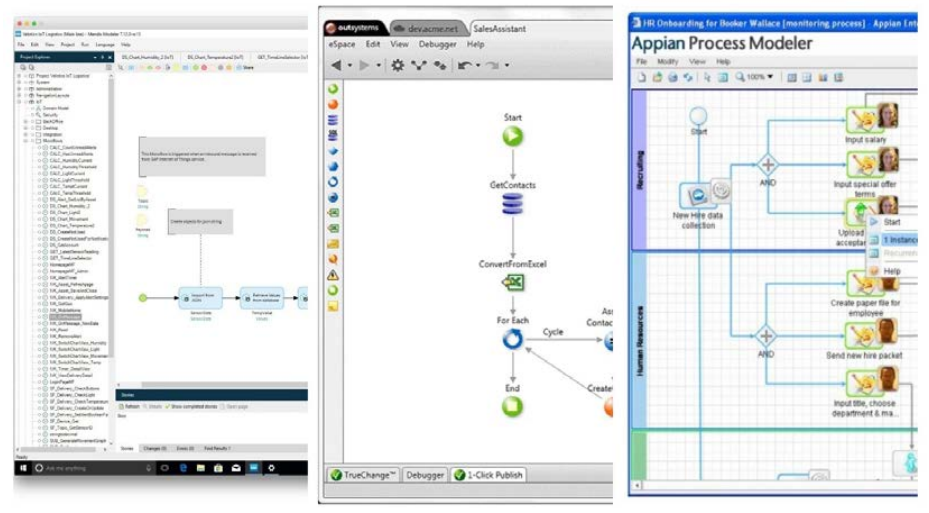
\includegraphics[width=0.9\textwidth]{LowCodePlatforms}
                \caption{LCDPs από αριστερά προς τα δεξιά: Mendix, OutSystems, Appian \cite{LowCodeMendix}}
        \end{figure}

        \subsection{Χαρακτηριστικά των LCDP}
            Παραθέτονται κάποια από τα χαρακτηριστικά που διακρίνουν τις πλατφόρμες ανάπτυξης σε Low-Code:

            \vspace{-0.5em}
            \begin{itemize}[label={\tiny \blacksquare}]
                \setlength\itemsep{-0.25em}
                \item \textbf{Γραφικό περιβάλλον χρήστη}: περιέρχονται εργαλεία και γραφικά στοιχεία, drag-and-drop χαρακτηριστικά, μηχανές αποφάσεων για τη μοντελοποίηση σύνθετης λογικής, κατασκευαστές φορμών (form builder)
                \item \textbf{Φορητότητα και συνεργασία}: επιτρέπουν στους χρήστες να εργάζονται από οποιαδήποτε τοποθεσία και οποιαδήποτε συσκευή ή λειτουργικό σύστημα.
                \item \textbf{Επεκτασιμότητα}: επαναχρησιμοποίηση προκατασκευασμένων στοιχείων, ύπαρξη marketplace και εύκολη ενσωμάτωση modules τρίτων.
                \item \textbf{Έλεγχος έκδοσης}: DevOps χαρακτηριστικά (για παράδειγμα σύστημα για version control όπως Git) και δυνατότητα για άμεσο deploy της εφαρμογής για το κοινό.
            \end{itemize}
            \vspace{-0.5em}

%        \subsection{Παραδείγματα LCDP}